% ============================================================
%  Springer LNCS Format — Smart Waste Segregation Paper
%  Compile with: pdflatex → bibtex → pdflatex → pdflatex
%  Or use Overleaf (recommended) — upload this file + llncs.cls
%  Download llncs.cls from:
%  https://www.springer.com/gp/computer-science/lncs/conference-proceedings-guidelines
% ============================================================

\documentclass[runningheads]{llncs}

% ── Packages ────────────────────────────────────────────────
\usepackage[T1]{fontenc}
\usepackage{graphicx}
\usepackage{booktabs}
\usepackage{amsmath}
\usepackage{amssymb}
\usepackage{multirow}
\usepackage{array}
\usepackage{url}
\usepackage{hyperref}
\usepackage{xcolor}
\usepackage{microtype}
\usepackage{float}
\usepackage{subcaption}

\hypersetup{
    colorlinks = true,
    linkcolor  = blue,
    citecolor  = blue,
    urlcolor   = blue
}

% ── Column type for centered fixed-width ────────────────────
\newcolumntype{C}[1]{>{\centering\arraybackslash}p{#1}}

% ============================================================
\begin{document}
% ============================================================

% ── Title ───────────────────────────────────────────────────
\title{BiFPN-Enhanced YOLO11s with Wise-IoU Loss\\
       for Real-Time Biodegradable Waste Detection}

\titlerunning{BiFPN-Enhanced YOLO11s for Waste Detection}

% ── Authors ─────────────────────────────────────────────────
\author{Minarul Hoque\inst{1} \and
        Rohan Dey\inst{1} \and
        Raktim Kumar\inst{1} \and
        Ataur Rahaman Din\inst{1} \and
        Rittwik Ghosh\inst{1} \and
        Debdutta Pal\inst{1}}

\authorrunning{Hoque et al.}

\institute{Department of Computer Applications,\\
           Adamas University, Kolkata, West Bengal, India\\
           \email{\{minarul1.haque,rohan1.dey,ritwik2.ghosh\}@stu.adamasuniversity.ac.in}\\
           \email{\{raktim1.kumar,ataur1.rahamanddin\}@stu.adamasuniversity.ac.in}\\
           \email{debdutta.pal1@adamasuniversity.ac.in}\\
           \url{https://adamasuniversity.ac.in}}

\maketitle

% ── Abstract ────────────────────────────────────────────────
\begin{abstract}
Rapid urbanisation has intensified the global solid waste crisis,
with over 2.01 billion tonnes of municipal solid waste generated
annually, yet source-level segregation remains critically low in most developing regions.
Manual sorting remains error-prone, inconsistent, and operationally
costly. This paper presents an automated real-time waste
detection system that localises and distinguishes biodegradable (\textit{Bio})
from non-biodegradable (\textit{Non-Bio}) waste using an enhanced
YOLO11s object detection architecture. Our approach incorporates
a Bidirectional Feature Pyramid Network (BiFPN) neck for improved
multi-scale feature fusion and a Wise-IoU (WIoU) loss function that
dynamically focuses on geometrically challenging bounding boxes.
Through systematic ablation experiments on the WasteManagement-2
dataset of 10,175 augmented images, we demonstrate that targeted
data augmentation yields the most significant performance improvement
(+15.0\% mAP@0.5), while BiFPN fusion further enhances multi-scale
feature representation. Our final model achieves \textbf{94.39\%}
mAP@0.5 on the validation set and \textbf{85.46\%} mAP@0.5 on the
held-out test set, at an inference speed of \textbf{4.0\,ms} per
image on an NVIDIA L40S GPU. Ablation studies reveal diminishing
returns from architectural complexity beyond BiFPN, guiding a
principled design toward a compact yet high-performing system.

\keywords{Waste Detection \and YOLO11 \and BiFPN \and
          WIoU Loss \and Object Detection \and Deep Learning \and
          Smart Waste Management}
\end{abstract}

% ============================================================
\section{Introduction}
% ============================================================

Municipal solid waste (MSW) management is one of the most pressing
environmental challenges of the twenty-first century. According to
the World Bank, global waste generation is projected to increase to
3.4 billion tonnes by 2050~\cite{worldbank2018}. Improper waste
disposal contributes to greenhouse gas emissions, soil contamination,
and public health hazards. Effective waste segregation at the point
of disposal—separating biodegradable organic matter from
non-biodegradable plastics, metals, and glass—is a critical first
step toward sustainable waste management, enabling composting,
recycling, and efficient landfill utilisation.

Conventional manual waste sorting is labour-intensive, subject to
human error (reported at over 20\% in uncontrolled
environments~\cite{systematic_review2025}), and impractical at
scale. Recent advances in deep learning, particularly in real-time
object detection, offer a promising avenue for automating waste
classification with high accuracy and minimal human intervention.

Convolutional neural network (CNN)-based approaches and YOLO-family
detectors have demonstrated strong performance in visual recognition
tasks, including waste identification~\cite{yolo_ec,ecodetect}.
However, challenges specific to waste classification—including high
intra-class visual variability, irregular object shapes, partial
occlusion, and overlapping waste items—demand architectural solutions
beyond standard detection pipelines.

In this work, we make the following \textbf{contributions}:
\begin{enumerate}
  \item We present a systematic eight-step ablation study quantifying
        the incremental impact of data augmentation, attention
        mechanisms (CBAM), feature pyramid enhancements (BiFPN), loss
        function variants (WIoU), and deformable convolutions~\cite{dai2017deformable} on
        waste detection performance.
  \item We propose a compact detection model combining YOLO11s~\cite{yolo11}
        with a BiFPN neck and WIoU v3 loss that achieves \textbf{94.39\%}
        mAP@0.5 on the validation set and \textbf{85.46\%} mAP@0.5
        on the held-out test set, with \textbf{4.0\,ms} GPU inference
        latency and a compact 19.2\,MB model size.
  \item We provide empirical evidence that strategic data augmentation
        is the dominant performance factor in waste detection tasks,
        outweighing architectural complexity gains.
  \item We release the \textbf{WasteManagement-2} dataset — 3,000
        manually annotated real-world images across mixed indoor and
        outdoor environments — under CC BY 4.0 as a public benchmark
        for binary waste detection research.
  \item We provide a \textbf{fully deployable real-time demo
        application} with webcam support, directly addressing the
        absence of deployment-ready open systems identified as a gap
        by recent surveys~\cite{springer_survey2024}.
\end{enumerate}

The remainder of this paper is organised as follows.
Section~\ref{sec:related} reviews related work.
Section~\ref{sec:method} describes the dataset, proposed architecture,
and training methodology.
Section~\ref{sec:experiments} presents experimental results and
ablation analysis.
Section~\ref{sec:conclusion} concludes with directions for future work.

% ============================================================
\section{Related Work}
\label{sec:related}
% ============================================================

\subsection{Early Deep Learning Approaches}

Automated waste classification gained research traction with
CNN-based approaches for distinguishing waste categories, including
foundational work on biodegradable versus non-biodegradable
classification~\cite{autoclassify2017}. Subsequent systems extended
this to lightweight CNN architectures suitable for embedded
deployment, demonstrating practical feasibility on resource-
constrained hardware.

\subsection{Hardware-Integrated Classification Systems}

Several works combine vision-based classification with physical
actuation hardware. An SSD-MobileNet model deployed on Raspberry Pi
achieved real-time bin-side waste detection at practical
latency~\cite{ssd_mobilenet2021}. ConvoWaste~\cite{convowaste2023}
combined a deep CNN classifier with servo-motor-actuated bin control
and ultrasonic fill-level sensors, demonstrating end-to-end automated
segregation. A 2024 study integrated VGG-16 and ResNet models with
IoT infrastructure, achieving improved classification on the TrashNet
dataset~\cite{iot_ai2024}. While these systems demonstrate
end-to-end deployment potential, they often trade classification
accuracy for hardware compatibility. In contrast, this work focuses
exclusively on maximising detection accuracy through architectural
optimisation, leaving physical actuation integration as future work.

\subsection{YOLO-Based Waste Detection}

The YOLO family of detectors has proven effective for real-time
waste detection. YOLO\_EC~\cite{yolo_ec} demonstrated that
augmentation strategies significantly improve detection of irregular
waste objects. EcoDetect-YOLO~\cite{ecodetect} introduced a
lightweight YOLO variant achieving real-time performance while
maintaining competitive accuracy. These works confirm that YOLO
architectures are well-suited to the waste classification domain,
motivating our choice of YOLO11s as the base detector.

\subsection{Feature Pyramid and Multi-Scale Methods}

BiFPN, introduced in EfficientDet~\cite{tan2020efficientdet},
applies bidirectional weighted feature fusion across pyramid levels,
enabling richer multi-scale representations at lower computational
cost than PANet variants. CBAM~\cite{woo2018cbam} provides channel
and spatial attention mechanisms that have shown benefit in general
object detection. While both components have been applied individually
in related domains, their specific utility and interaction in binary
waste classification — where objects span multiple scales, textures,
and high intra-class variability — has not been systematically
evaluated prior to this work. Our ablation study provides the first
controlled assessment of CBAM's impact on this task.

\subsection{Comparative Summary}

Table~\ref{tab:related} summarises the reviewed works alongside the
proposed method. Results are reported on each study's own dataset and
are therefore not directly numerically comparable; the table is
intended to illustrate methodological differences rather than
rank absolute performance.

\begin{table}[H]
\centering
\caption{Comparison of Related Works}
\label{tab:related}
\renewcommand{\arraystretch}{1.05}
\resizebox{\linewidth}{!}{%
\begin{tabular}{l l l l c l}
\toprule
\textbf{Study} & \textbf{Dataset} & \textbf{Task} & \textbf{Model} &
\textbf{Classes} & \textbf{Best Result / Limitation} \\
\midrule
Sudha et al.~\cite{autoclassify2017}    & Custom (lab)        & Classification & CNN              & 2      & Proof-of-concept; no localization \\
Koganti et al.~\cite{ssd_mobilenet2021} & Custom              & Detection      & SSD-MobileNet    & 2      & $\sim$82\% mAP; embedded-only \\
Nafiz et al.~\cite{convowaste2023}      & Custom              & Classification & DCNN             & Multi  & $\sim$89\% acc.; single-item only \\
Alourani et al.~\cite{iot_ai2024}       & TrashNet            & Classification & ResNet-50        & 6      & 91.4\% acc.; no bounding boxes \\
Fan et al.~\cite{yolo_ec}              & HPU\_WASTE           & Detection      & YOLO\_EC         & Multi  & 96.4\% mAP; no ablation study \\
Liu et al.~\cite{ecodetect}            & Custom domestic     & Detection      & Lightweight YOLO & Multi  & $\sim$87\% mAP; accuracy--efficiency trade-off \\
\midrule
\textbf{Ours} & \textbf{WasteManagement-2} & \textbf{Detection} &
\textbf{YOLO11s+BiFPN+WIoU} & \textbf{2} &
\textbf{94.4\% mAP@0.5 (val) / 85.5\% (test)} \\
\bottomrule
\end{tabular}}
\end{table}

\subsection{Research Gaps}

A 2025 systematic review analysing 97 studies~\cite{systematic_review2025}
found that deep learning-based systems consistently outperform
traditional computer vision approaches, with YOLO-family detectors
leading in real-time deployment. A parallel survey of 45 smart dustbin
implementations~\cite{springer_survey2024} independently recommends
YOLO-family architectures as the current state-of-the-art for
camera-based intelligent waste systems. Despite this progress, key
gaps remain: (i) most systems evaluate on controlled, single-item
datasets; (ii) systematic ablation studies isolating individual
architectural contributions are rare; (iii) few works rigorously
compare augmentation strategies against architectural innovations.
This work directly addresses these gaps.

% ============================================================
\section{Proposed Methodology}
\label{sec:method}
% ============================================================

\subsection{Dataset}

We constructed a custom waste image dataset comprising \textbf{3,000
raw images} across two classes: \textit{Bio} (biodegradable organic
waste) and \textit{Non-Bio} (non-biodegradable waste including
plastics, metals, and glass). Images were collected through a
combination of direct photography using mobile cameras and targeted
internet collection, covering both indoor and outdoor environments
to ensure diversity in lighting, background, and waste presentation
conditions.

All images were manually annotated using the Roboflow platform,
producing bounding box labels for each waste instance. A subset of
272 label files contained polygon (segmentation) annotations rather
than the 5-field YOLO bounding box format required for training.
These were corrected by computing, for each polygon, the tightest
axis-aligned bounding box from the minimum and maximum of its
normalised coordinate sequence — preserving the full object extent
without any manual re-annotation. Additionally, one duplicate image
and within-file duplicate annotation lines were removed to prevent
double-counting during loss computation. After these fixes, all
3,000 images carried clean, consistent YOLO-format labels. The
annotated dataset is publicly available on Roboflow Universe
under CC BY 4.0 at: \url{https://universe.roboflow.com/minaruls-workspace-2ptiz/wastemanagement-3iq6q-hl0ll/dataset/2}

To improve generalisation, we applied a structured augmentation
pipeline exclusively to the \textbf{training split} via Roboflow v2,
expanding the training set from 2,387 unique source images to
\textbf{9,576 images} (average $\times$4.01 augmentation factor).
Validation and test splits retain only the original unaugmented
images, ensuring no augmented copy of a validation or test image
appears in training. The augmentation operations applied were:
horizontal flip (50\% probability), random rotation ($\pm15°$),
brightness jitter ($\pm20\%$), exposure jitter ($\pm15\%$), and
mosaic augmentation. All images were resized to $640\times640$ pixels
with auto-orientation. Dataset composition is summarised in
Table~\ref{tab:dataset}.

\begin{table}[H]
\centering
\caption{WasteManagement-2 Dataset Composition}
\label{tab:dataset}
\begin{tabular}{lrrrr}
\toprule
\textbf{Split} & \textbf{Images} & \textbf{Bio Boxes} & \textbf{Non-Bio Boxes} & \textbf{Total Boxes} \\
\midrule
Train      & 9,576  & 18,834 & 20,228 & 39,062 \\
Validation & 300    & 179    & 177    & 356    \\
Test       & 299    & 267    & 255    & 522    \\
\midrule
\textbf{Total} & \textbf{10,175} & \textbf{19,280} & \textbf{20,660} & \textbf{39,940} \\
\bottomrule
\end{tabular}
\end{table}

\subsection{Base Architecture: YOLO11s}

We adopt \textbf{YOLO11s}~\cite{yolo11} (small variant) as our
base detector, selected through preliminary comparisons against
YOLOv8n and YOLO11n. YOLO11s employs C3k2 blocks in the backbone, providing a
favourable trade-off between parameter efficiency and feature
extraction capacity. The fused model contains 101 layers,
9,413,574 parameters, and 21.3\,GFLOPs, with a model size of
19.2\,MB—compact for deployment on standard GPU-equipped hardware,
with potential for further optimisation toward edge deployment.

\subsection{BiFPN Neck}

Standard Feature Pyramid Networks (FPN) fuse features in a single
top-down direction, limiting their ability to propagate information
across scales. We replace the standard neck with a
\textbf{Bidirectional Feature Pyramid Network
(BiFPN)}~\cite{tan2020efficientdet}, which applies bidirectional
(top-down and bottom-up) feature fusion with learnable scalar
weights. The weighted fusion at each BiFPN node is computed as:

\begin{equation}
  \mathcal{O} = \frac{\sum_{i} w_i \cdot I_i}{\sum_{i} w_i + \varepsilon},
  \label{eq:bifpn}
\end{equation}

\noindent where $w_i$ are learnable non-negative weights normalised
via ReLU and $\varepsilon = 10^{-4}$ ensures numerical stability.
We configure BiFPN with $\text{channels}=256$ and 2 fusion
iterations, operating on feature maps P3 ($80\times80$),
P4 ($40\times40$), and P5 ($20\times20$).

In the context of waste classification, BiFPN provides richer
representations of both large items (bins, bags) and small objects
(bottle caps, wrappers), which appear at different pyramid scales.

\subsection{Wise-IoU Loss v3 (WIoU v3)}

Standard IoU-based losses treat all bounding box predictions
equally, giving the same gradient weight to easy and hard examples.
We adopt \textbf{Wise-IoU v3 (WIoU v3)}~\cite{wiou2023}, the
dynamic-focusing variant that computes a per-example weight $\beta$
based on how each prediction's IoU compares to the batch mean IoU:

\begin{equation}
  \mathcal{L}_{\text{WIoU}} = \beta \cdot \mathcal{L}_{\text{IoU}}, \quad
  \beta = \left(\frac{\text{IoU}_i}{\overline{\text{IoU}}}\right)^{\!4},
  \label{eq:wiou}
\end{equation}

\noindent where $\text{IoU}_i$ is the IoU of the $i$-th prediction
and $\overline{\text{IoU}}$ is the batch mean IoU. Predictions with
IoU below the batch mean (hard examples) receive $\beta < 1$,
focusing gradient updates on geometrically challenging boxes while
down-weighting easy, already well-aligned predictions. In our
implementation, $\text{IoU}_i$ is clamped to $[0.01, 1.0]$ and
$\beta$ to $[0.1, 10.0]$ for numerical stability during early
training. For waste objects with irregular, partially occluded
shapes, this mechanism provides more informative gradient signals
than standard IoU loss.

\subsection{Overall Architecture}

The complete proposed system is illustrated in
Fig.~\ref{fig:architecture}. An RGB input image ($640\times640\times3$)
is processed through the YOLO11s backbone, producing multi-scale
feature maps P3, P4, and P5. These are fused bidirectionally by the
BiFPN neck and passed to an anchor-free detection head that predicts
class labels, confidence scores, and bounding boxes, optimised with
WIoU loss.

\begin{figure}[H]
  \centering
  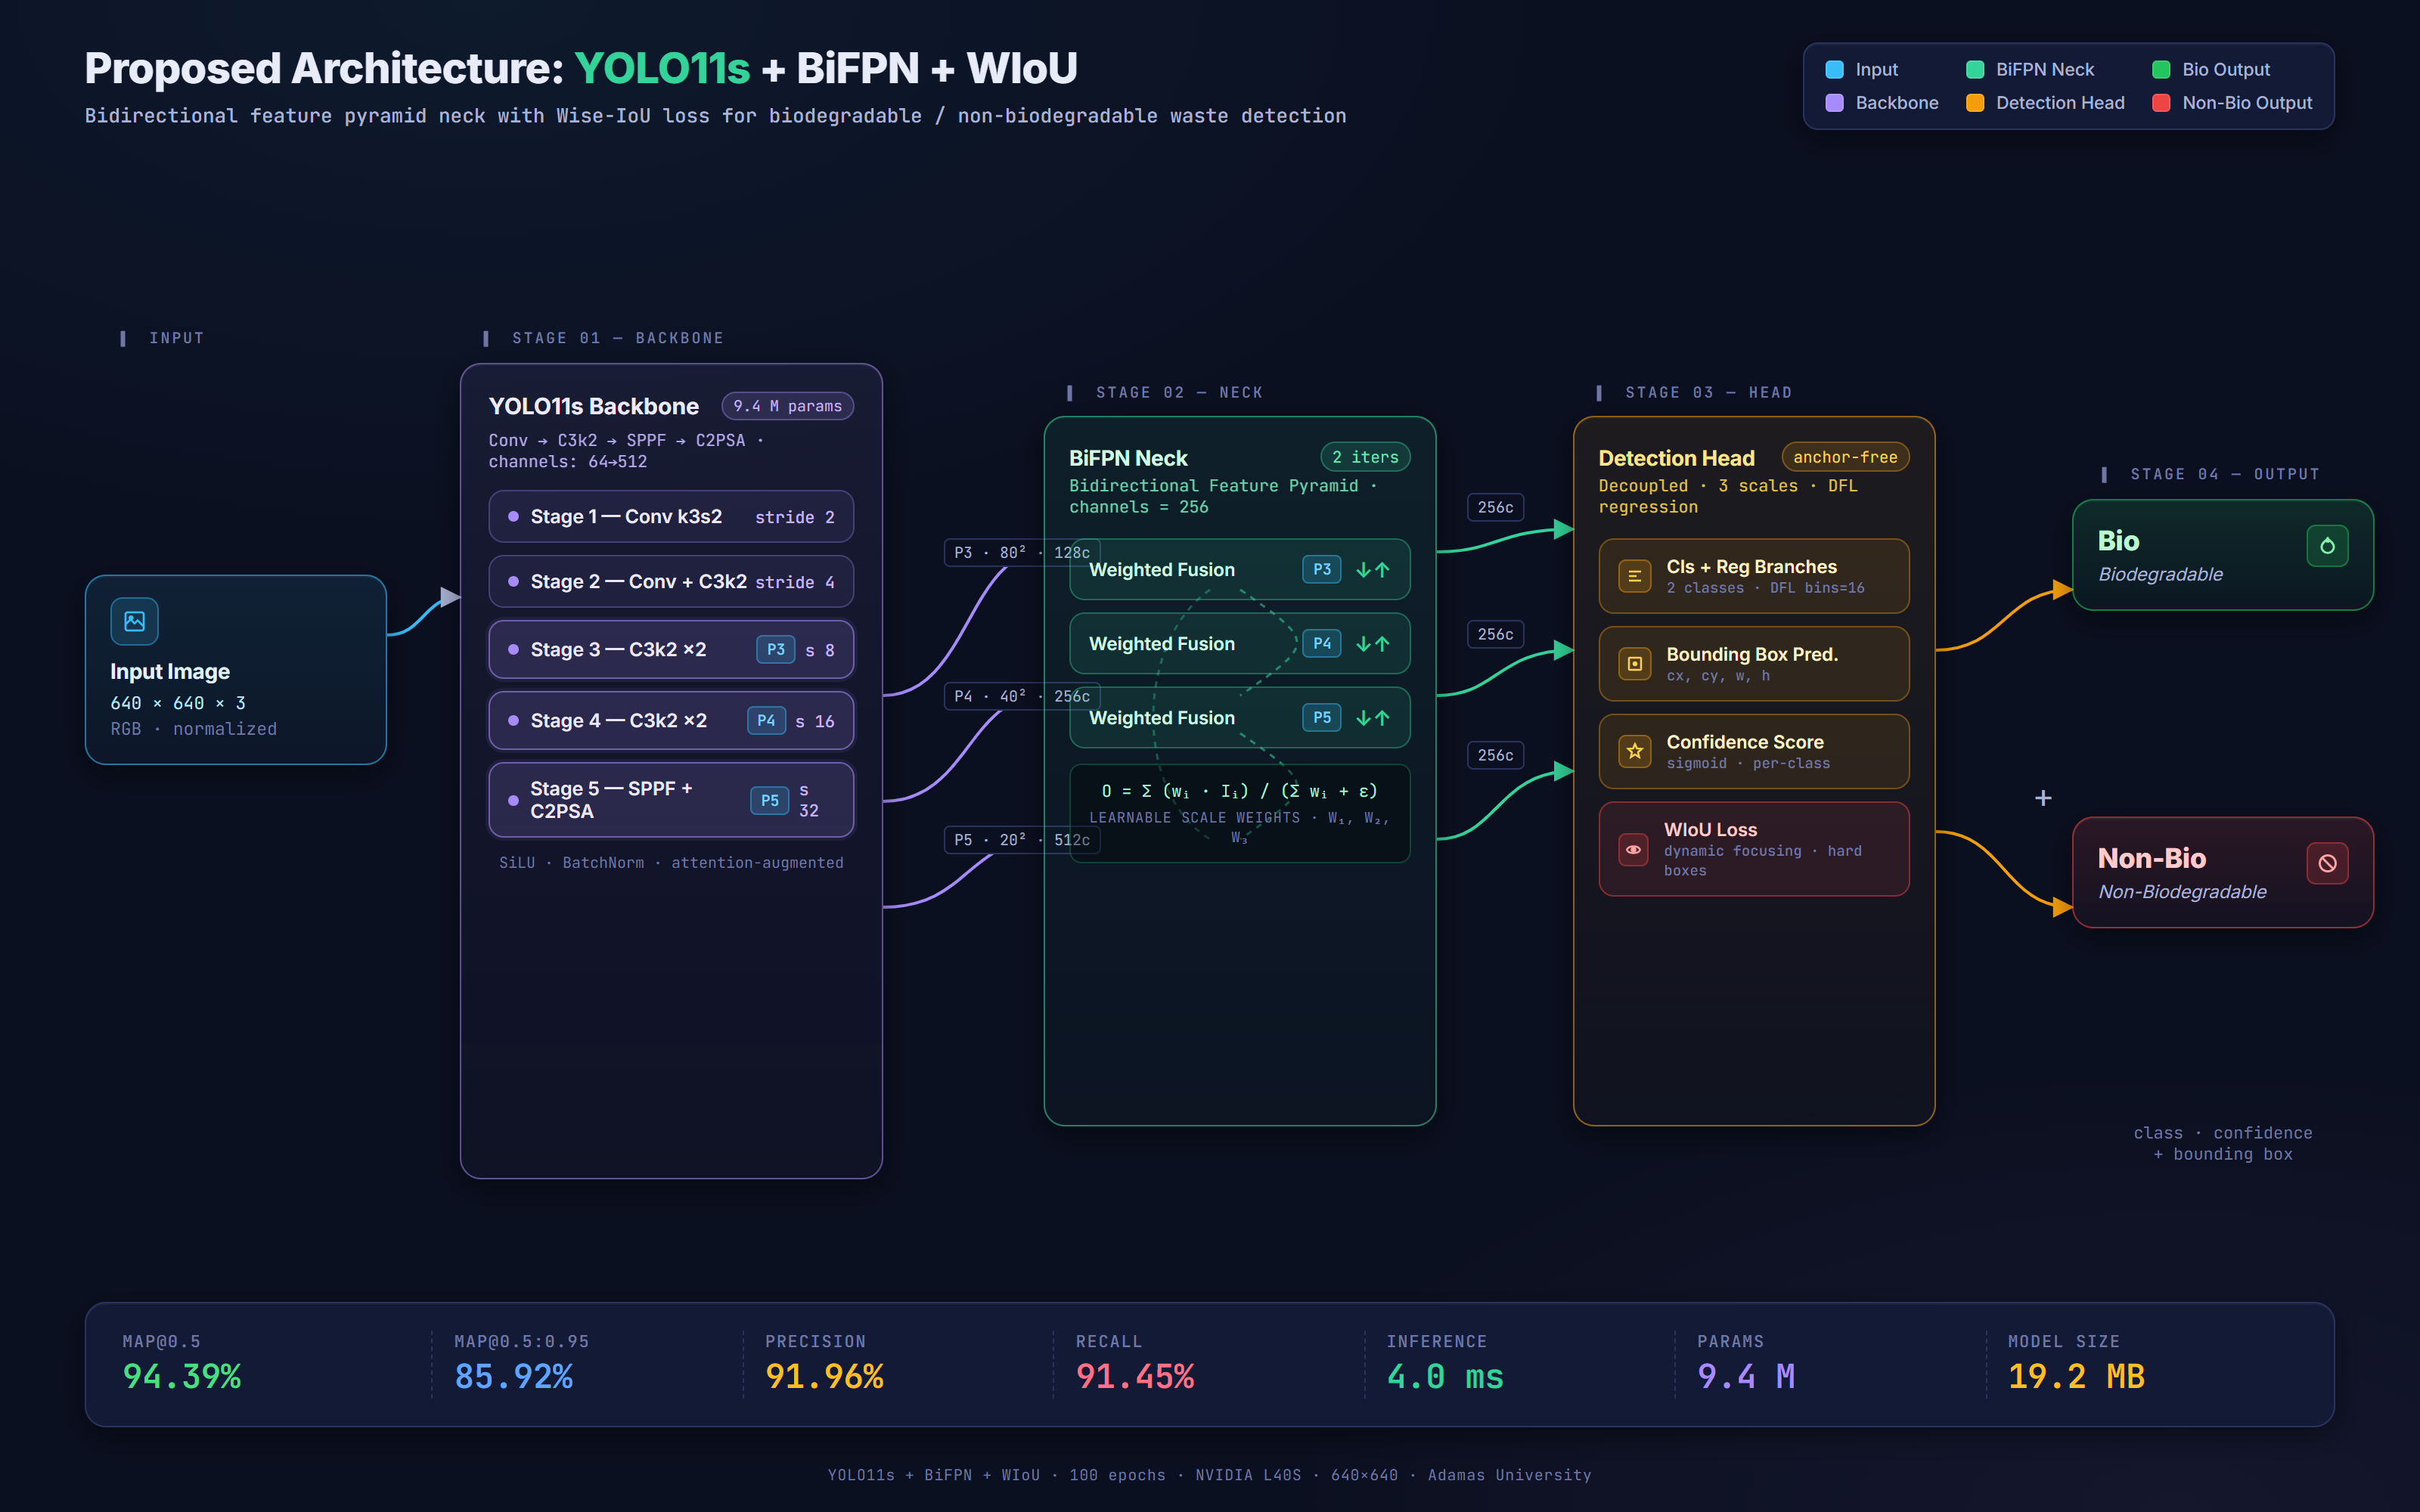
\includegraphics[width=\textwidth]{architecture_diagram.png}
  \caption{Proposed architecture: YOLO11s backbone with BiFPN neck
           and WIoU v3-optimised anchor-free detection head for
           real-time binary waste detection.}
  \label{fig:architecture}
\end{figure}

\subsection{Training Configuration}

All experiments were conducted on an NVIDIA L40S GPU (46\,GB VRAM).
The final model training configuration is summarised in
Table~\ref{tab:training}.

\begin{table}[H]
\centering
\caption{Final Training Hyperparameters}
\label{tab:training}
\begin{tabular}{ll}
\toprule
\textbf{Parameter}     & \textbf{Value} \\
\midrule
Base model             & YOLO11s (COCO pretrained) \\
Epochs                 & 100 \\
Batch size             & 32 \\
Image size             & $640 \times 640$ \\
Optimizer              & AdamW~\cite{loshchilov2019adamw} \\
Initial LR ($lr_0$)    & 0.01 \\
Final LR ($lr_f$)      & 0.001 \\
LR schedule            & Cosine annealing \\
Warmup epochs          & 3 \\
Weight decay           & 0.0005 \\
Loss function          & WIoU (bounding box) \\
BiFPN channels         & 256 (2 iterations) \\
Total training time    & 3.102 hours \\
\bottomrule
\end{tabular}
\end{table}

% ============================================================
\section{Experiments and Results}
\label{sec:experiments}
% ============================================================

\subsection{Evaluation Metrics}

We evaluate all models using standard COCO detection metrics:
\textbf{mAP@0.5} (mean Average Precision at IoU threshold 0.50),
\textbf{mAP@0.5:0.95} (mean AP averaged over IoU thresholds
0.50--0.95 at step 0.05), \textbf{Precision} (P), \textbf{Recall}
(R), and GPU inference speed in milliseconds per image. Ablation
comparisons use the 300-image validation set (356 instances). Final
model performance is additionally evaluated on the held-out 299-image
test set (522 instances) to provide an unbiased performance estimate.

\subsection{Ablation Study}

We conducted a systematic eight-step ablation study to quantify
the contribution of each architectural component. Results are
presented in Table~\ref{tab:ablation}.

\begin{table}[H]
\centering
\caption{Ablation Study Results on WasteManagement-2 Validation Set}
\label{tab:ablation}
\setlength{\tabcolsep}{5pt}
\renewcommand{\arraystretch}{1.1}
\begin{tabular}{c p{6.2cm} c r r}
\toprule
\textbf{Step} & \textbf{Configuration} & \textbf{Ep.} &
\textbf{mAP@.5} & \textbf{mAP@.5:.95} \\
\midrule
1 & YOLO11n, no augmentation          & 50  & 0.7566 & \multicolumn{1}{c}{$-$} \\
2 & YOLO11s, no augmentation          & 50  & 0.7565 & \multicolumn{1}{c}{$-$} \\
3 & YOLO11s + Augmentation            & 50  & 0.9060 & \multicolumn{1}{c}{$-$} \\
4 & YOLO11s + Aug + CBAM + WIoU       & 50  & 0.8805 & 0.7420 \\
5 & YOLO11s + Aug + BiFPN + CBAM + WIoU & 50 & 0.9159 & 0.7934 \\
6 & Step 5 + Deformable Convolutions  & 50  & 0.8812 & 0.7448 \\
\midrule
7 & YOLO11s + Aug + BiFPN + WIoU (no CBAM) & 50  & 0.8877 & 0.7550 \\
\textbf{8} & \textbf{YOLO11s + Aug + BiFPN + WIoU} & \textbf{100} &
\textbf{0.9439} & \textbf{0.8592} \\
\bottomrule
\end{tabular}
\end{table}

\noindent The ablation study yields five key findings:

\begin{itemize}
  \item \textbf{Finding 1 — Data augmentation is the dominant factor.}
        Steps 2$\to$3 yield $+15.0\%$ absolute mAP@0.5 improvement,
        representing the single largest performance gain across all
        interventions, exceeding all architectural modifications
        combined.

  \item \textbf{Finding 2 — BiFPN improves multi-scale fusion.}
        BiFPN (Step 5: 91.59\%) provides a meaningful gain over the
        augmented baseline (Step 3: 90.60\%), confirming that
        bidirectional feature fusion better represents the multi-scale
        nature of waste objects.

  \item \textbf{Finding 3 — Deformable convolutions are detrimental.}
        Step 6 (88.12\%) decreases performance relative to Step 5
        (91.59\%), demonstrating that architectural complexity beyond
        BiFPN introduces optimisation difficulty without representational
        benefit on this dataset scale.

  \item \textbf{Finding 4 — Architecture vs.\ training-time effects are
        separable.} Step 7 evaluates the final architecture (BiFPN +
        WIoU, CBAM removed) at 50 epochs, yielding 88.77\% mAP@0.5.
        This is below Step 5 (91.59\%), confirming that the CBAM removal
        trades short-term performance for lower initialisation overhead.
        Step 8 trains the same architecture to 100 epochs, recovering and
        surpassing all 50-epoch baselines at 94.39\%.

  \item \textbf{Finding 5 — Extended training contributes $+5.62\%$
        mAP@0.5.} The gain from Step 7 (88.77\%, 50 ep) to Step 8
        (94.39\%, 100 ep) isolates the training-time contribution,
        confirming the BiFPN + WIoU architecture continues improving
        without overfitting across 100 epochs.
\end{itemize}

\noindent\textbf{CBAM exclusion rationale.}
CBAM degraded performance when first introduced (Step 4: 88.05\%,
$-2.55\%$ vs.\ augmented baseline) and, while it partially recovered
when combined with BiFPN (Step 5: 91.59\%), it was ultimately
excluded from the final model for two reasons. First, waste images
exhibit high intra-class texture variability — organic matter,
soiled packaging, and mixed debris present irregular, noisy feature
patterns — making channel and spatial suppression by attention
potentially counterproductive. Second, CBAM introduces additional
initialisation overhead when loading from COCO pretrained weights,
creating a feature distribution mismatch at the attention gates that
requires extended training to overcome; within a 50-epoch budget
this manifests as slower convergence. Removing CBAM and instead
extending training to 100 epochs yields a net gain of $+2.80\%$
over the best CBAM-included model, confirming that the initialisation
overhead was the binding constraint, not the attention mechanism's
representational capacity per se.

\subsection{Final Model Performance}

Table~\ref{tab:final} presents the per-class evaluation of our
final model on both the validation set (used for architecture
selection) and the held-out test set (independent evaluation).

\begin{table}[H]
\centering
\caption{Final Model Performance — YOLO11s + BiFPN + WIoU (100 Epochs)}
\label{tab:final}
\setlength{\tabcolsep}{4pt}
\begin{tabular}{lcccc|cc}
\toprule
 & \multicolumn{4}{c|}{\textbf{Validation Set (300 images)}} &
   \multicolumn{2}{c}{\textbf{Test Set (299 images)}} \\
\textbf{Class} & \textbf{P} & \textbf{R} & \textbf{AP@0.5} &
\textbf{AP@0.5:0.95} & \textbf{AP@0.5} & \textbf{AP@0.5:0.95} \\
\midrule
Bio     & 0.8960 & 0.9195 & 0.9362 & 0.8310 & 0.7745 & $-$ \\
Non-Bio & 0.9432 & 0.9096 & 0.9517 & 0.8260 & 0.9348 & $-$ \\
\midrule
\textbf{Overall} & \textbf{0.9196} & \textbf{0.9145} &
\textbf{0.9439} & \textbf{0.8592} & \textbf{0.8546} & \textbf{0.7709} \\
\bottomrule
\end{tabular}
\end{table}

On the validation set the model achieves \textbf{94.39\% mAP@0.5}
with strong per-class balance (Bio: 93.62\%, Non-Bio: 95.17\%).
On the held-out test set — which is more densely annotated
(522 instances across 299 images vs.\ 356 in validation) — the model
achieves \textbf{85.46\% mAP@0.5}. The Non-Bio class maintains high
test accuracy (93.48\%), while the Bio class shows greater
sensitivity to the harder test distribution (77.45\%), likely due to
the higher visual variability of organic waste under real-world
conditions. GPU inference runs at \textbf{4.0\,ms per image}
($\approx$250\,FPS on the NVIDIA L40S), well within the 50\,ms
real-time threshold. All inference benchmarks were obtained on the
L40S training GPU; deployment on lower-power hardware would require
additional profiling.

\subsection{Confusion Matrix and Precision-Recall Analysis}

Figure~\ref{fig:confusion} shows the normalised confusion matrix on the
validation set. Both classes achieve high true-positive rates, with
minimal cross-class confusion. The slightly higher false-positive rate
for the Bio class is consistent with the greater intra-class visual
variability of organic waste items.

\begin{figure}[H]
  \centering
  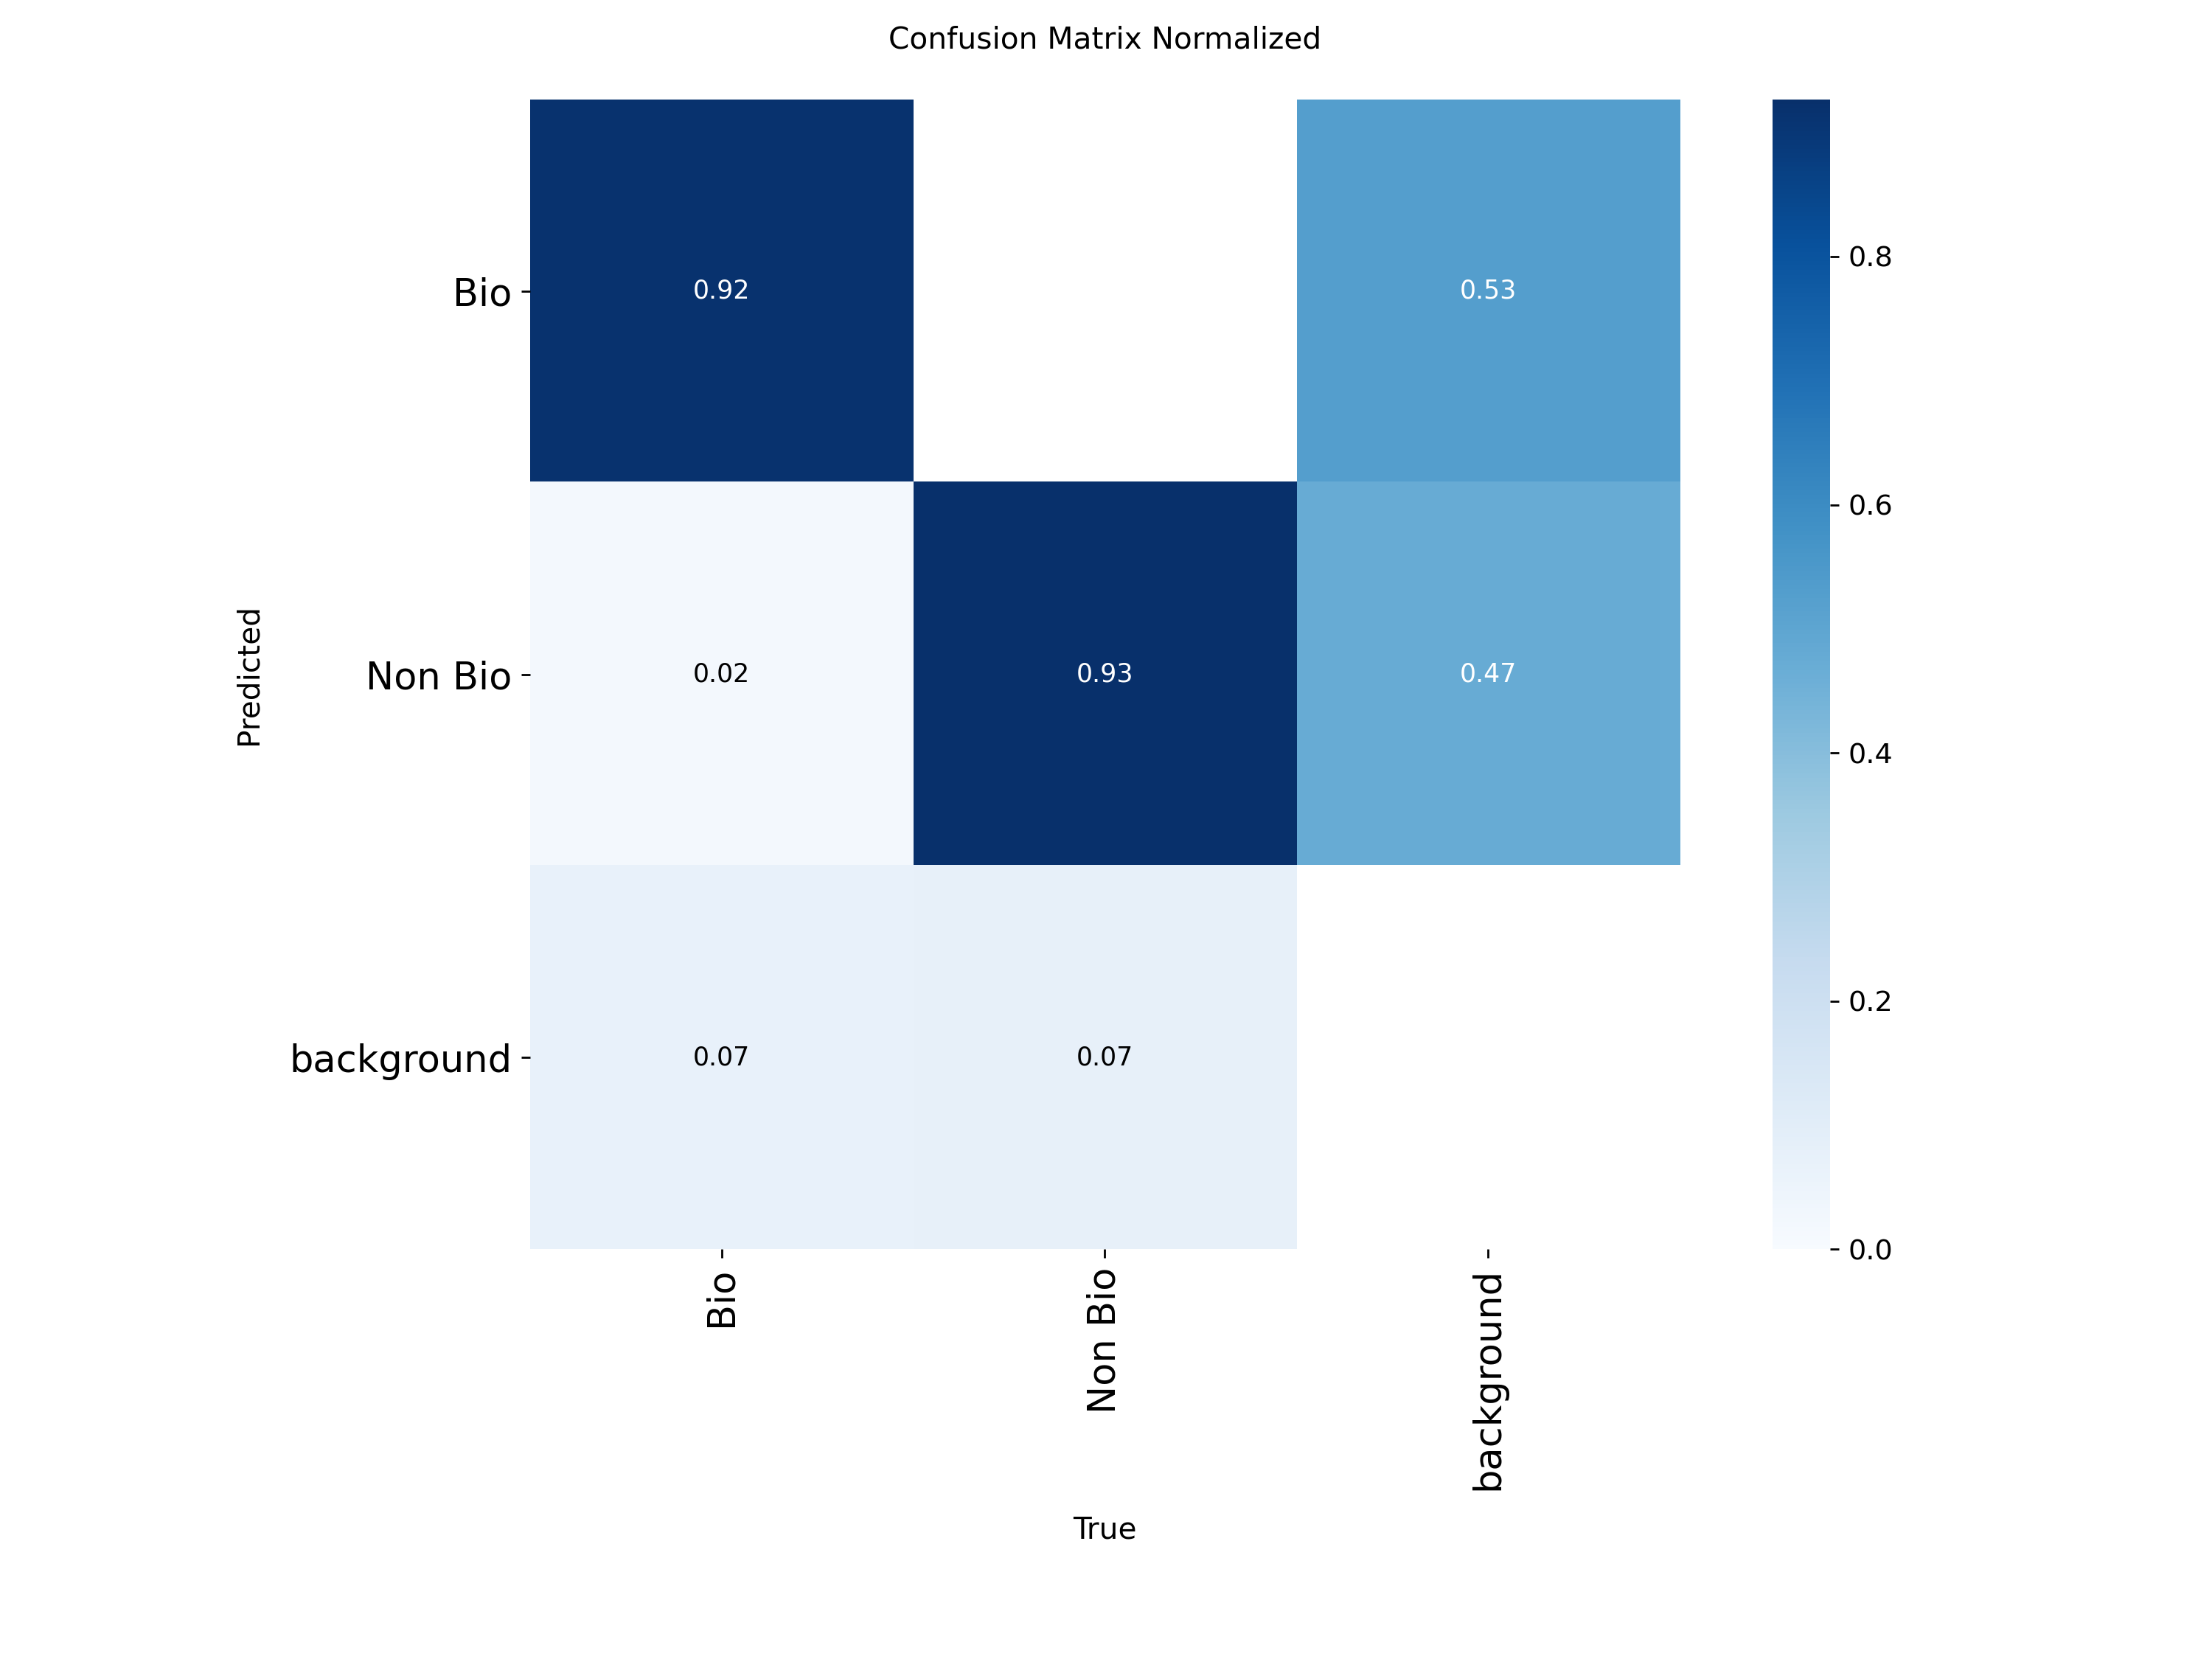
\includegraphics[width=0.72\textwidth]{confusion_matrix_normalized.png}
  \caption{Normalised confusion matrix — final model on the 300-image
           validation set. Rows are ground-truth classes; columns are
           predicted classes.}
  \label{fig:confusion}
\end{figure}

Figure~\ref{fig:pr} presents the per-class Precision-Recall curves.
Both classes maintain high precision across a wide recall range,
confirming reliable detections without excessive false positives even
at aggressive confidence thresholds. The area under each curve
corresponds directly to the reported AP@0.5 values: 93.62\% (Bio) and
95.17\% (Non-Bio).

\begin{figure}[H]
  \centering
  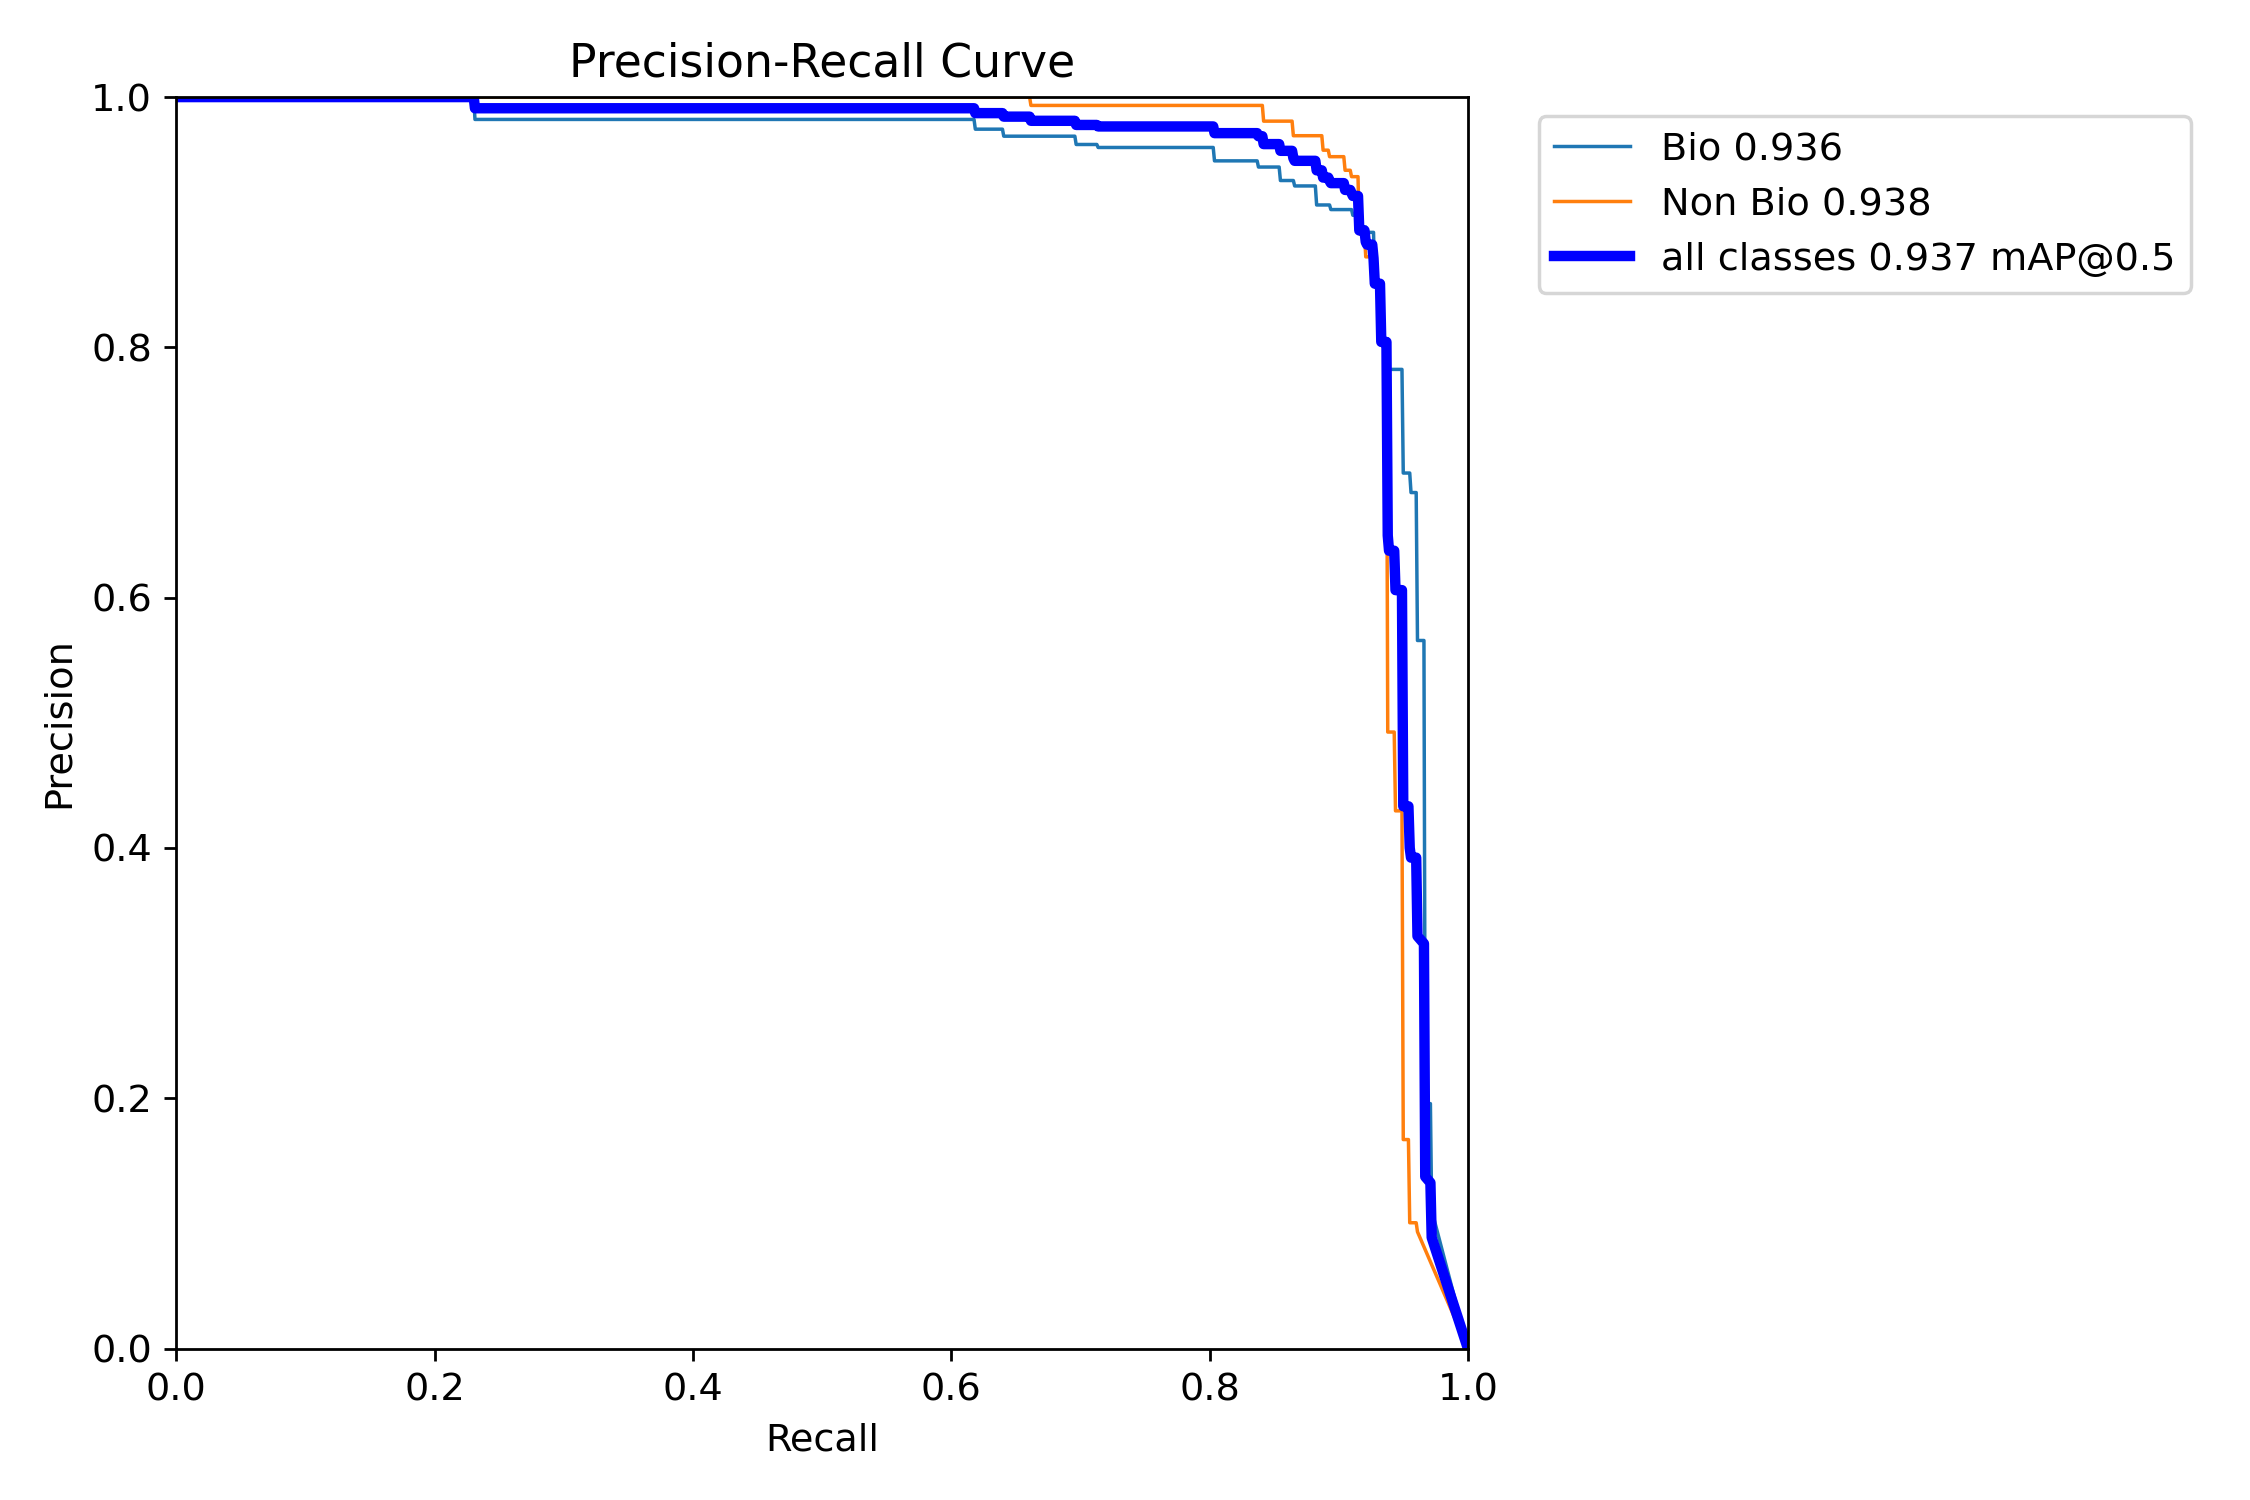
\includegraphics[width=0.82\textwidth]{BoxPR_curve.png}
  \caption{Precision-Recall curves for Bio and Non-Bio classes.
           mAP@0.5 = 94.39\% (overall), shown as the dashed line.}
  \label{fig:pr}
\end{figure}

\subsection{Qualitative Detection Results}

Figure~\ref{fig:qualitative} shows representative detection outputs
from the final model across four distinct scenarios: isolated
Non-Bio waste, isolated Bio waste, a mixed-class scene, and a
densely cluttered multi-item image. The model correctly localises
and classifies waste items across varying scales, backgrounds, and
occlusion levels, demonstrating practical robustness beyond
aggregate metric performance.

% ── Replace the four \rule placeholders below with actual detection
%    screenshots once captured from the demo application.
%    Recommended filenames (place in same folder as this .tex file):
%    qual_nonbio.jpg  |  qual_bio.jpg  |  qual_mixed.jpg  |  qual_multi.jpg
\begin{figure}[htbp]
\centering
\begin{subfigure}[b]{0.47\textwidth}
  
\includegraphics[width=\textwidth]{plastic_bag.png}
  \caption{Non-Bio: plastic bag detected}
\end{subfigure}
\hfill
\begin{subfigure}[b]{0.47\textwidth}
  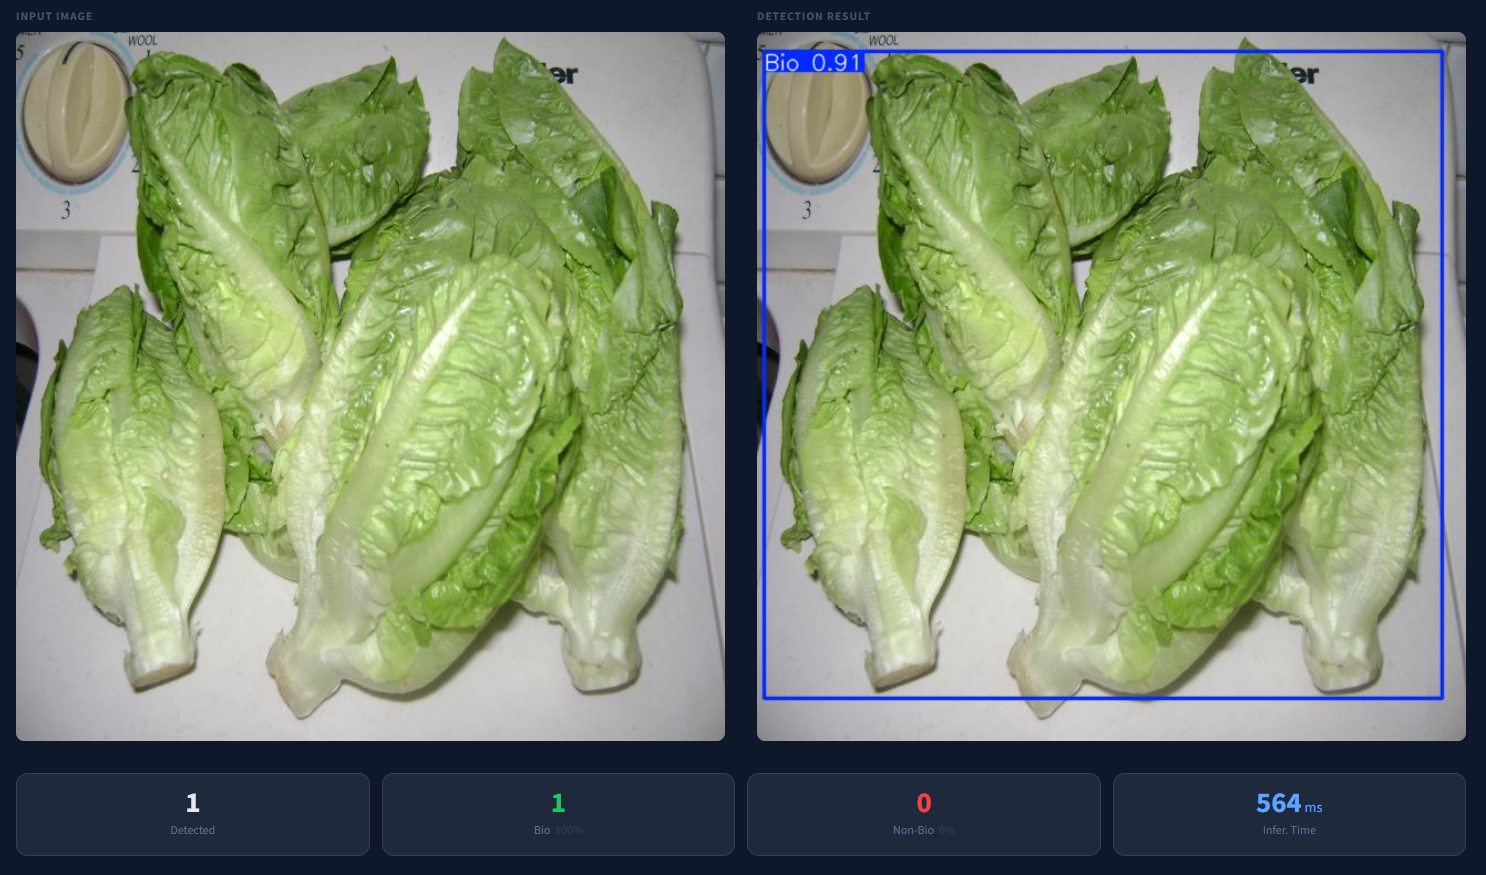
\includegraphics[width=\textwidth]{organic.png}
  \caption{Bio: organic waste detected}
\end{subfigure}
\\[0.5em]
\begin{subfigure}[b]{0.47\textwidth}
  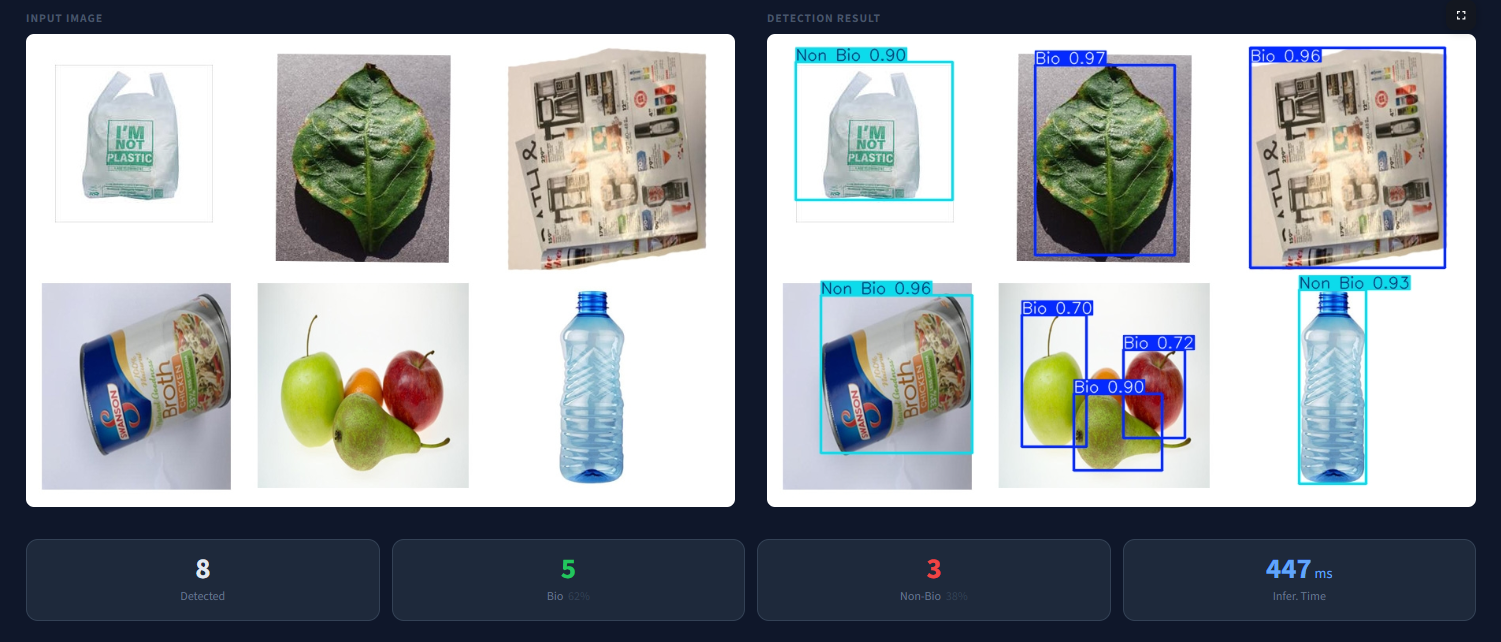
\includegraphics[width=\textwidth]{multiple_items.png}
  \caption{Multiple items: Bio + Non-Bio co-detected}
\end{subfigure}
\hfill
\begin{subfigure}[b]{0.47\textwidth}
  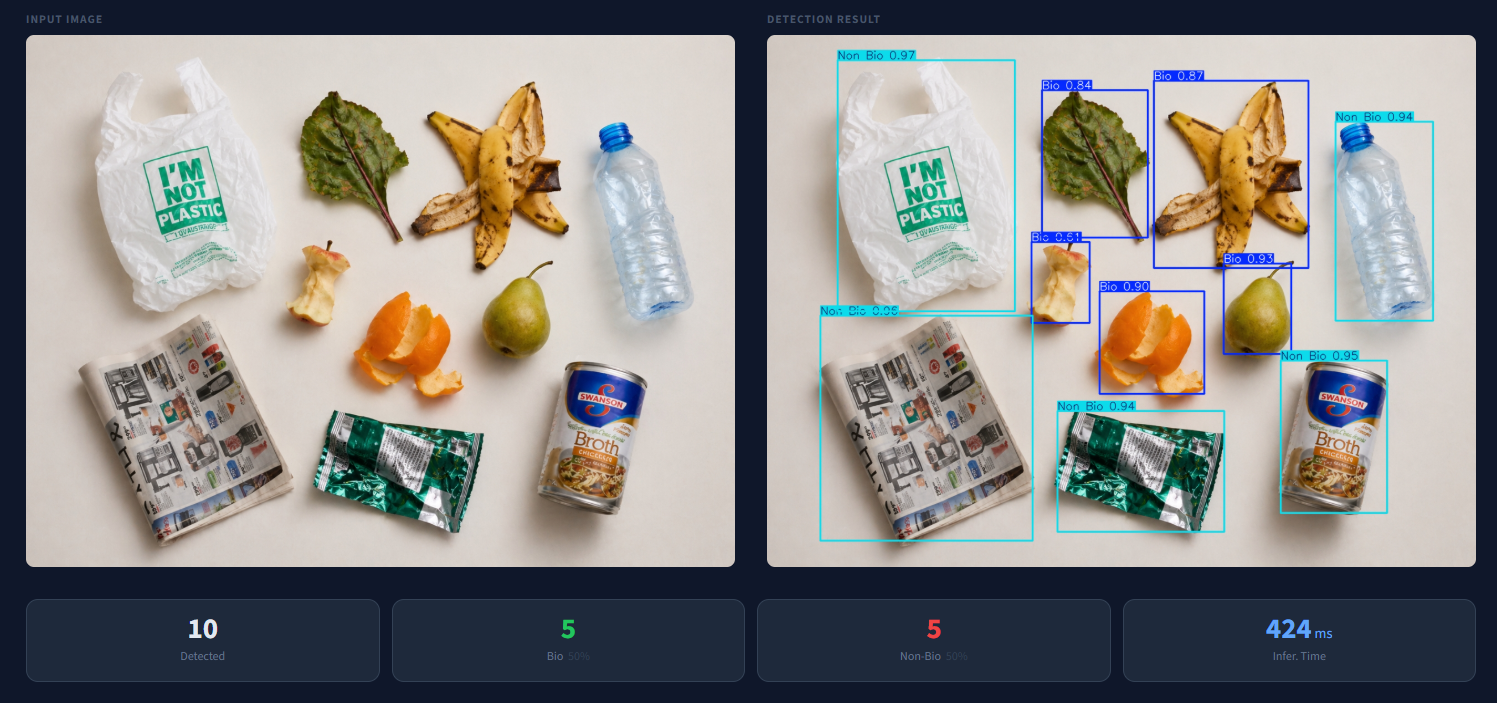
\includegraphics[width=\textwidth]{cluttered_items.png}
  \caption{Cluttered scene: dense multi-item detection}
\end{subfigure}
\caption{Qualitative detection results from the final YOLO11s + BiFPN
         + WIoU v3 model across four real-world scenarios.
         Green boxes indicate \textit{Bio}; red boxes indicate
         \textit{Non-Bio}. Confidence scores shown above each box.}
\label{fig:qualitative}
\end{figure}

\subsection{Comparison with Baseline Models}

Table~\ref{tab:comparison} compares our final model against standard
YOLO baseline variants trained under identical conditions on the
same dataset.

\begin{table}[H]
\centering
\caption{Comparison Across YOLO Variants (same dataset, 50-epoch baselines)}
\label{tab:comparison}
\begin{tabular}{lccc}
\toprule
\textbf{Model} & \textbf{mAP@0.5} & \textbf{Precision} & \textbf{Recall} \\
\midrule
YOLOv8n                         & 0.7631 & $-$ & $-$    \\
YOLO11n                        & 0.7566 & $-$ & 0.6646 \\
YOLO11s                        & 0.7565 & $-$ & 0.7132 \\
YOLO11s + Augmentation         & 0.9060 & $-$ & 0.8400 \\
\midrule
\textbf{Ours (YOLO11s + BiFPN + WIoU, 100ep)} &
\textbf{0.9439} & \textbf{0.9196} & \textbf{0.9145} \\
\bottomrule
\end{tabular}
\end{table}

Our final model outperforms all baseline variants by a substantial
margin, demonstrating the combined benefit of augmentation, BiFPN
feature fusion, WIoU loss, and extended training.

% ============================================================
\section{Conclusion}
\label{sec:conclusion}
% ============================================================

This paper presented a systematic investigation into deep
learning-based binary waste detection for automated segregation
into biodegradable and non-biodegradable categories. We proposed an
enhanced YOLO11s detector incorporating a BiFPN neck and WIoU v3
bounding box loss, trained on the augmented WasteManagement-2
dataset of 10,175 images.

Our eight-step ablation study yielded three principal findings. First,
data augmentation is the single most impactful intervention,
contributing over 15\% absolute mAP improvement. Second, BiFPN-based
bidirectional feature fusion provides meaningful gains in multi-scale
waste detection. Third, additional architectural complexity — such as
deformable convolutions — yields no benefit and may degrade
performance, indicating a point of diminishing returns beyond BiFPN.

The final model achieves \textbf{94.39\% mAP@0.5} on the validation
set and \textbf{85.46\% mAP@0.5} on the held-out test set, with
\textbf{4.0\,ms} GPU inference latency and a compact 19.2\,MB model
size, demonstrating practical feasibility for automated waste
segregation systems. The observed gap between validation and test
performance — attributable to the more densely annotated and visually
diverse test partition — highlights Bio class detection as the primary
direction for future improvement.

Future work will explore: (i) multi-category classification beyond
binary segregation; (ii) integration with physical bin actuation
hardware for end-to-end validation; (iii) model distillation for
microcontroller-class edge deployment; and (iv) continual learning
strategies for adapting to new waste categories without full
retraining.

% ── Acknowledgements ────────────────────────────────────────
\section*{Acknowledgements}
The authors thank the Department of Computer Applications, Adamas
University, for providing access to the NVIDIA L40S GPU infrastructure
used in this study.

% ============================================================
%  References
% ============================================================
\bibliographystyle{splncs04}

\begin{thebibliography}{99}

\bibitem{yolo11}
Ultralytics:
{YOLO11}: A New Era in Object Detection.
Ultralytics (2024).
\url{https://docs.ultralytics.com/models/yolo11/}

\bibitem{worldbank2018}
Kaza, S., Yao, L., Bhada-Tata, P., Van Woerden, F.:
What a Waste 2.0: A Global Snapshot of Solid Waste Management to 2050.
World Bank Group, Washington DC (2018).
\url{https://doi.org/10.1596/978-1-4648-1329-0}

\bibitem{convowaste2023}
Nafiz, M.S., Das, S.S., Morol, M.K., Juabir, A.A., Nandi, D.:
ConvoWaste: An automatic waste segregation machine using deep learning.
In: Proceedings of the International Conference on Research in
Engineering, Science and Technology (ICREST) (2023).
\url{https://doi.org/10.48550/arXiv.2302.02976}

\bibitem{ssd_mobilenet2021}
Koganti, S.K., Purnima, G., Bhavana, P., Raghava, Y.V., R., Resmi:
Deep learning based automated waste segregation system based on
degradability.
In: 2021 Second International Conference on Electronics and Sustainable
Communication Systems (ICESC), pp.~1953--1956 (2021).
\url{https://doi.org/10.1109/icesc51422.2021.9532837}

\bibitem{autoclassify2017}
Sudha, S., Vidhyalakshmi, M., Pavithra, K., Sangeetha, K., Swadhikar, V.:
An automatic classification method for environment-friendly waste
segregation using deep learning.
In: 2016 International Conference on Advanced Communication Control and
Computing Technologies (ICACCCT) (2016).
\url{https://ieeexplore.ieee.org/document/7801215/}

\bibitem{iot_ai2024}
Alourani, A., Ashraf, M.U., Aloraini, M.:
Smart waste management and classification system using advanced
{IoT} and {AI} technologies.
PeerJ Computer Science \textbf{11}, e2777 (2025).
\url{https://doi.org/10.7717/peerj-cs.2777}

\bibitem{systematic_review2025}
Noor, R.M., Hijazi, M.S., Ahmedy, I., Ismail, N.M., Daud, S.:
A systematic review of artificial intelligence-based techniques
for solid waste management.
Sensors \textbf{25}(10), 3181 (2025).
\url{https://doi.org/10.3390/s25103181}

\bibitem{yolo_ec}
Fan, J., Cui, L., Fei, S.:
Waste detection system based on data augmentation and {YOLO\_EC}.
Sensors \textbf{23}(7), 3646 (2023).
\url{https://doi.org/10.3390/s23073646}

\bibitem{ecodetect}
Liu, S., Chen, R., Ye, M., Luo, J., Yang, D., Dai, M.:
{EcoDetect-YOLO}: A lightweight, high-generalisation methodology for
real-time detection of domestic waste exposure in intricate
environmental landscapes.
Sensors \textbf{24}(14), 4666 (2024).
\url{https://doi.org/10.3390/s24144666}

\bibitem{tan2020efficientdet}
Tan, M., Pang, R., Le, Q.V.:
EfficientDet: Scalable and efficient object detection.
In: Proceedings of the IEEE/CVF Conference on Computer Vision
and Pattern Recognition (CVPR), pp.~10781--10790 (2020).
\url{https://doi.org/10.1109/CVPR42600.2020.01079}

\bibitem{woo2018cbam}
Woo, S., Park, J., Lee, J.Y., Kweon, I.S.:
CBAM: Convolutional block attention module.
In: Proceedings of the European Conference on Computer Vision
(ECCV), pp.~3--19 (2018).
\url{https://doi.org/10.1007/978-3-030-01234-2_1}

\bibitem{wiou2023}
Tong, Z., Chen, Y., Xu, Z., Yu, R.:
Wise-{IoU}: Bounding box regression loss with dynamic focusing mechanism.
arXiv preprint arXiv:2301.10051 (2023).
\url{https://doi.org/10.48550/arXiv.2301.10051}

\bibitem{springer_survey2024}
Arthur, M.P., Shoba, S., Pandey, A.:
A survey of smart dustbin systems using the {IoT} and deep learning.
Artificial Intelligence Review \textbf{57} (2024).
\url{https://doi.org/10.1007/s10462-023-10646-6}

\bibitem{dai2017deformable}
Dai, J., Qi, H., Xiong, Y., Li, Y., Zhang, G., Hu, H., Wei, Y.:
Deformable convolutional networks.
In: Proceedings of the IEEE International Conference on Computer
Vision (ICCV), pp.~764--773 (2017).
\url{https://doi.org/10.1109/ICCV.2017.89}

\bibitem{loshchilov2019adamw}
Loshchilov, I., Hutter, F.:
Decoupled weight decay regularization.
In: International Conference on Learning Representations (ICLR) (2019).
\url{https://openreview.net/forum?id=Bkg6RiCqY7}

\end{thebibliography}

\end{document}
